
\chapter{Aspectos Técnicos}\label{chapter:technical}

La implementación de un sistema de memoria robótica asume que muchos sistemas y capacidades de un robot están disponibles. Entonces, se requiere del uso de variados frameworks y librerías que permiten comunicarse con el robot y acceder a los datos de interés que se desea recordar. En este capítulo se presenta el software de interés para la implementación de la memoria y se detalla la plataforma objetivo.

% ================================================================
% ================================================================
% ================================================================

\section{ROS}

Los sistemas robóticos actuales son cada vez más complejos. Deben lidiar con muchos componentes tanto de hardware como de software y su interacción, de una forma eficaz y que no entorpezca el desarrollo. Muchas tareas de control requieren altas frecuencias de funcionamiento, así como la sincronización y comunicación entre los diversos módulos. Por lo tanto, el cómo se unen los subsistemas en una aplicación robótica es una tarea difícil.

ROS \cite{ROS:2009}, acrónimo para Robot Operating System, es un proyecto que funciona como middleware para aplicaciones robóticas, y permite resolver el problema de la comunicación entre procesos. Es una colección de herramientas, librerías y convenciones que buscan simplificar la tarea de crear comportamientos robóticos complejos y robustos, sin importar la plataforma robótica.

Fue originalmente creado por la organización WillowGarage en el 2008, y mantenido actualmente por la Open Source Robotics Foundation (OSRF). Existe un ecosistema ROS, mantenido por la comunidad, y con cientos de módulos de software con soluciones a problemas específicos, los que pueden interconectarse para construir comportamientos más complejos. Por lo anterior, su uso se ha convertido en una práctica mundial, siendo adoptado incluso en soluciones industriales.

%\todo[inline]{Más información sobre ROS. Lo que sea relevante para la implementación y el diseño.}

%\subsubsection{Nodo}
%
%Mensajes y master
%
%\subsubsection{Tópicos}
%
%\subsubsection{Servicios}
%
%\subsubsection{Servidor de parámetros}
%
%\subsubsection{Launch}

%\subsubsection{Herramientas}

%\subsubsection{Actionlib}


%\subsection{SMACH}

%\todo[inline]{Sobre librería para máquinas de estado (a utilizar en la demostración)}


\subsection{UChile ROS Framework}

UChile ROS Framework (URF) hace referencia al sistema de software desarrollado en el laboratorio de robótica del Departamento de Ingeniería Eléctrica de la Universidad de Chile, para sus robots de servicio. El sistema cuenta con 10 años de desarrollo y está orientado a cumplir los requisitos de la competencia Robocup en su categoría @Home.

URF está construido sobre ROS y en una estructura de 4 capas. La primera capa contiene todas las dependencias del sistema, ya sean de ROS o no; Es la única capa donde que contiene código externo. Sobre ella, se monta una capa ROS de bajo nivel, con herramientas y librerías comunes, sumado a los drivers necesarios para manejar cada robot. La capa intermedia alberga capacidades robóticas avanzadas, relacionadas a percepción robótica, manipulación de objetos, navegación autónoma e interacción Humano-Robot. Finalmente, existe una capa desarrollada en python, con interfaces para el uso de las capacidades de menor nivel, utilizada para la elaboración de maquinas de estado y comportamientos robóticos complejos.

\begin{figure}[H]
\centering
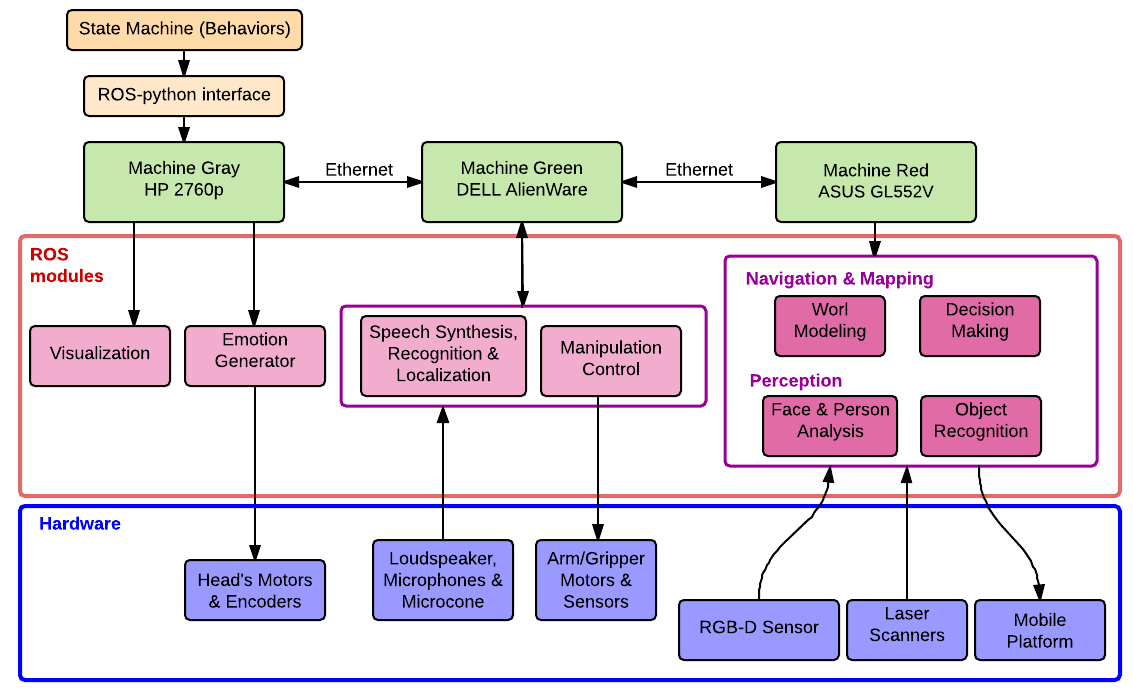
\includegraphics[width=0.8\textwidth]{./figures/URF.png}
\caption{\small Diagrama de UChile ROS Framework utilizado en el robot Bender.}
\label{img:URF}
\end{figure}

Todos los módulos de URF son de código libre, a excepción de los algoritmos relacionados con percepción y la interfaz de alto nivel. El código se almacena públicamente en la organización \textit{uchile-robotics} en GitHub\footnote{Organización \textit{uchile-robotics} y URF en GitHub: \url{https://github.com/uchile-robotics}}.


%\subsubsection{Concepto de robot-skills}
\todo[inline]{Sobre concepto de robot skills y cómo permiten acceder a componentes del robot. Serán utilizadas para la demo.}


\subsubsection{Manejo de información en URF}

Si un robot implementa URF, entonces es posible acceder a la información compartida por sus procesos. Cualquier módulo ROS en el sistema tiene acceso a los datos extraídos desde sensores y luego generados en post-procesamientos, junto al acceso para controlar el hardware.

Existen algunas formas de memoria implementadas en URF, comparables a los conceptos definidos para la memoria humana. También se pueden dividir en de corto y largo plazo:

Como STM, se puede definir como memoria de trabajo a todo el flujo de información presente durante la ejecución del robot. Lo que incluye datos sensados, procesamientos y acciones realizadas. Generalmente tales datos no son almacenados para posteriores ejecuciones.

A manera de LTM, se puede encontrar una memoria procedural, relacionada con todo el conocimiento almacenado que posee el robot para cumplir ciertas tareas. Caen en esta categoría: modelos para percepción robótica, modelos para reconocimiento de voz y patrones, bases de datos de movimientos precalculados para manipular objetos y acciones predefinidas que se utilizan para controlar el robot.

También se pueden encontrar especializaciones de memoria LTM semántica. Ejemplos de esto son: El mapa que se conoce del entorno, junto a los lugares y objetos anotados en él. Diccionarios con información anotada sobre entidades y sus características, cómo personas y objetos. Bases de datos con imágenes anotadas para el reconocimiento de objetos y personas. 

Sin embargo, en URF no existen formas de memoria emocional ni episódica de largo plazo. Luego, toda interacción realizada por los robots está limitada a la información obtenida desde el inicio al término de cada rutina.



\subsection{KnowRob}

KnowRob es un sistema de procesamiento de conocimiento. Combina métodos para representar conocimiento y para razonar a partir de él, junto a técnicas  para adquirir conocimiento y almacenarlo físicamente. Permite integrar información proveniente de distintas fuentes \cite{Tenorth2013, Tenorth2009}.

Está implementado en Java y Prolog, y provee una interfaz ROS. Almacena los datos en archivos OWL (Web Ontology Language) y en una base de datos NoSQL, MongoDB. Por su diseño, permite el manejo e inferencia de memoria semántica y procedural.


\todo[inline]{Más info sobre knowRob... todo el trabajo se basará en este software!.}

\todo[inline]{Sobre OWL... utilizado por KnowRob.}

\todo[inline]{Sobre Prolog... utilizado por KnowRob.}

\todo[inline]{Sobre MongoDB... utilizada por KnowRob.}

% ================================================================
% ================================================================
% ================================================================


\section{Plataforma objetivo: Robot Bender}

Bender es un robot humanoide creado el año 2007 en el laboratorio de robótica del Departamento de Ingeniería Eléctrica de la Universidad de Chile. El equipo UChile Homebreakers es el encargado de su desarrollo y  su objetivo es ser un mayordomo para el hogar, funcionando de manera autónoma para apoyar en tales labores \cite{uchile-robotics}.

\begin{figure}[H]
\centering
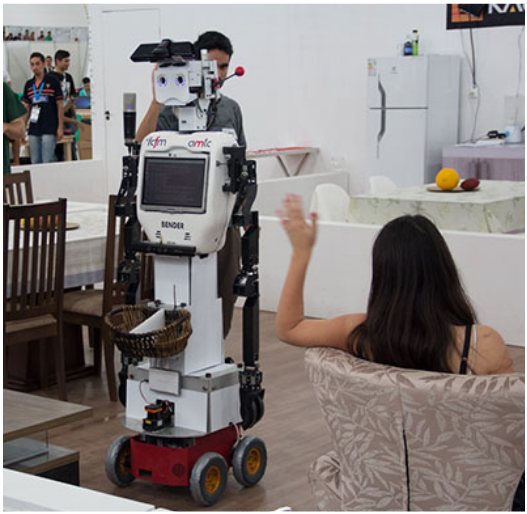
\includegraphics[width=0.5\textwidth]{./figures/bender.png}
\caption{\small Robot Bender en competencia RoboCup 2015.}
\label{img:bender}
\end{figure}


En cuanto a actuadores, el robot cuenta con 2 brazos antropomórficos de 6 grados de libertad cada uno, una base móvil diferencial Pioneer 3-AT, un cuello que permite rotaciones en dos ejes cartesianos; pudiendo imitar gestos de asentimiento y negación, y finalmente, una cabeza que puede mostrar expresiones faciales mediante movimientos de su boca, orejas, cejas y cambios de colores alrededor de los ojos.

El robot cuenta con los siguientes sensores: un laser Hokuyo UTM-30LX, un laser Hokuyo URG-04LX-UG01, un micrófono M-Audio Producer USB y una cámara de profundidad ASUS Xtion Pro.

El software de Bender está basado en el framework URF. Su arquitectura de software utiliza  ROS para el manejo de componentes de bajo y medio nivel. La capa de alto nivel, escrita en python, se abstrae de ROS y permite la creación de comportamientos complejos mediante máquinas de estado. Todos los módulos que interactúan con sensores y actuadores están implementados en ROS.



%\todo[inline]{Robot pepper es eliminado por ahora, para acotar los alcances.}
%\subsection{Pepper}
%
%Pepper es un robot humanoide desarrollado por SoftBank Robotics, orientado a la interacción humano robot y con el objetivo de ser un robot de compañía y soporte emocional.


%\section{Contribución del Trabajo}



